\chapter{Calculus, Differential Equations and Numerical Integration}
\label{ch:calculus}
\chaptermark{Calculus and ODEs} % short running header

\begin{objectives}
\begin{itemize}
  \item Use partial derivatives, gradients, Jacobians and Hessians, and the chain rule in matrix form.
  \item Use Taylor's theorem with explicit error terms; this is what ``linearization'' and ``first order'' mean.
  \item Differentiate common matrix expressions: inverses, quadratic forms, determinants.
  \item Solve linear ordinary differential equations, including time-varying ones, with the state transition matrix.
  \item Integrate differential equations numerically, predict the order of the error, and verify it.
  \item Compute derivatives numerically with a step size chosen from first principles.
\end{itemize}
\end{objectives}

A navigation filter is a differential equation (the vehicle's motion) integrated numerically from noisy derivatives (the IMU
readings), corrected with linearized measurement models. This chapter collects the calculus behind those three activities:
derivatives and linearization, differential equations and their solutions, and the numerical methods that approximate both.

% ==============================================================================
\section{Derivatives of functions of several variables}

\subsection{Partial derivatives, gradients and Jacobians}

For a scalar function $f(x_1, \dots, x_n)$, the \emph{partial derivative} $\partial f/\partial x_j$ is the ordinary derivative with respect to
$x_j$ with the other variables held fixed. The \term{gradient} collects them:
$\nabla f = (\partial f/\partial x_1, \dots, \partial f/\partial x_n)\T$. For a vector function $f: \R^n \to \R^m$ the partial derivatives form the
\term{Jacobian} matrix.

\begin{definition}[Jacobian, numerator layout]
For $f: \R^n \to \R^m$, the Jacobian $\frac{\partial f}{\partial x} \in \R^{m\times n}$ has entries
$\big[\frac{\partial f}{\partial x}\big]_{ij} = \frac{\partial f_i}{\partial x_j}$. Row $i$ is the gradient of the $i$-th output (transposed); column $j$ is
the sensitivity of all outputs to the $j$-th input.
\end{definition}

The Jacobian is the matrix of the best linear approximation of $f$ near $x$:
\begin{equation}
  f(x + \delta) = f(x) + \frac{\partial f}{\partial x}\,\delta + o(\|\delta\|),
  \label{eq:linearization}
\end{equation}
where $o(\|\delta\|)$ denotes a remainder that goes to zero faster than $\|\delta\|$. Column $j$ is exactly what a finite-difference
test computes by perturbing the $j$-th input (\cref{sec:numdiff}).

\begin{proposition}[Chain rule]
\label{prop:chain-rule}
\index{chain rule}
If $y = f(x)$ and $z = g(y)$, then $\dfrac{\partial z}{\partial x} = \dfrac{\partial g}{\partial y}\Big|_{y = f(x)}\,\dfrac{\partial f}{\partial x}$.
\end{proposition}
\begin{proof}
Substitute the linear approximation of $f$ into that of $g$:
$g(f(x + \delta)) = g\big(f(x) + J_f\delta + o(\|\delta\|)\big) = g(f(x)) + J_gJ_f\delta + o(\|\delta\|)$.
\end{proof}

With the numerator layout the factors appear in the same order as the composition $g\circ f$, which makes long chains easy to write: the
Jacobian of a camera measurement with respect to a pose is ``(projection) times (frame change) times (pose perturbation)''
(\cref{ch:msckfupdate}).

The \term{Hessian} of a scalar function is the matrix of second derivatives, $[\nabla^2f]_{ij} = \partial^2f/\partial x_i\partial x_j$. For smooth $f$ it is
symmetric. It describes curvature: the second-order behavior of $f$ near a point.

\subsection{Taylor's theorem}

\begin{theorem}[Taylor's theorem in one variable]
\label{thm:taylor}
\index{Taylor's theorem}
If $f$ has $n + 1$ continuous derivatives, then
\begin{equation}
  f(x + h) = \sum_{k=0}^n\frac{f^{(k)}(x)}{k!}h^k + \frac{f^{(n+1)}(\xi)}{(n+1)!}h^{n+1}
\end{equation}
for some $\xi$ between $x$ and $x + h$ (Lagrange form of the remainder).
\end{theorem}

The theorem says more than ``$f$ is close to its Taylor polynomial'': it bounds the error. If $|f^{(n+1)}| \le M$ on the interval, the
error of the degree-$n$ polynomial is at most $Mh^{n+1}/(n+1)!$. This is how we will judge every approximation in these notes.

\begin{figure}[t]
  \centering
  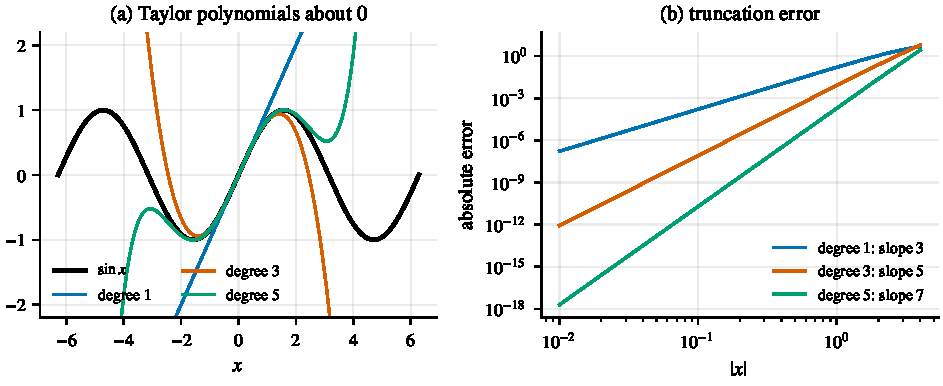
\includegraphics[width=0.95\textwidth]{fig_taylor_sin.pdf}
  \caption{Taylor polynomials of $\sin x$ about $0$ (left) and the absolute error of each (right, log-log scale). Near the expansion point the
  error of the degree-$n$ polynomial falls like $|x|^{n+1}$ or faster. Because the even-order terms of $\sin x$ vanish, the polynomials of degree 1, 3
  and 5 coincide with those of degree 2, 4 and 6, and their errors fall like $|x|^3$, $|x|^5$ and $|x|^7$ (slopes 3, 5 and 7). Far from the
  expansion point, every truncated series fails.}
  \label{fig:taylor-sin}
\end{figure}

\paragraph{Big-O and little-o.} We write $g(h) = O(h^p)$ if $|g(h)| \le Ch^p$ for some constant $C$ as $h\to0$, and $g(h) = o(h^p)$ if
$g(h)/h^p \to 0$. An approximation is \emph{first-order accurate} if its error is $O(h^2)$: the error of a linearization shrinks
quadratically with the size of the perturbation. ``Keeping terms to first order'' in a derivation means writing the result as
linear terms plus an $O(\|\delta\|^2)$ remainder, and then dropping the remainder.

For functions of several variables, Taylor's theorem to second order reads
\begin{equation}
  f(x + \delta) = f(x) + \nabla f(x)\T\delta + \tfrac12\delta\T\nabla^2f(x)\,\delta + O(\|\delta\|^3),
\end{equation}
and for vector functions each component expands this way. The size of the second-order term relative to the first measures how good a
linearization is: when uncertainties are small compared with the scale over which the Jacobian changes, linearization is accurate.
This is the quantitative content of the statement that an extended Kalman filter works well when errors are small (\cref{ch:nonlinear}).

\subsection{Matrix calculus}

A few derivatives recur throughout estimation. We write them as differentials ($\dd f$ = the linear change of $f$ for a small change of the
argument):
\begin{align}
  \dd(Ax) &= A\,\dd x, & \frac{\partial (Ax)}{\partial x} &= A, \\
  \dd(x\T Ax) &= x\T(A + A\T)\,\dd x, & \nabla_x(x\T Ax) &= (A + A\T)x \ \ (= 2Ax \text{ if } A \text{ symmetric}), \\
  \dd(a\times x) &= \sx{a}\,\dd x, & \dd(x \times a) &= -\sx{a}\,\dd x, \\
  \dd(A\inv) &= -A\inv(\dd A)A\inv, & \dd\log\det A &= \tr(A\inv\dd A) .
\end{align}
\begin{proof}[Derivations]
The first and third lines are linear maps, their own derivatives. For the quadratic form,
$(x + \dd x)\T A(x + \dd x) - x\T Ax = \dd x\T Ax + x\T A\,\dd x + O(\|\dd x\|^2) = x\T(A\T + A)\dd x + O(\|\dd x\|^2)$. For the inverse,
differentiate $AA\inv = I$: $(\dd A)A\inv + A\,\dd(A\inv) = 0$. For the log-determinant of a positive-definite $A = U\Lambda U\T$, a small
change $\dd A$ changes each eigenvalue by $u_i\T(\dd A)u_i$ to first order, so
$\dd\sum_i\log\lambda_i = \sum_iu_i\T(\dd A)u_i/\lambda_i = \tr(U\Lambda\inv U\T\dd A) = \tr(A\inv\dd A)$.
\end{proof}

\subsection{Stationary points}

A smooth function has a local minimum at $x^\star$ only if $\nabla f(x^\star) = 0$, and it does have one if, in addition,
$\nabla^2f(x^\star) \succ 0$: by the second-order Taylor expansion, $f(x^\star + \delta) - f(x^\star) = \tfrac12\delta\T\nabla^2f\,\delta + O(\|\delta\|^3) > 0$
for small $\delta \neq 0$. Every least-squares problem in these notes is solved by setting a gradient to zero; \cref{ch:nlls} develops the
iterative methods needed when the resulting equations are nonlinear.

% ==============================================================================
\section{Ordinary differential equations}

\subsection{What a differential equation is}

An \term{ordinary differential equation} (ODE) in state-space form is
\begin{equation}
  \dot x(t) = f\big(x(t), t\big), \qquad x(t_0) = x_0,
\end{equation}
where $x(t) \in \R^n$ is the \emph{state} and $\dot x = \dd x/\dd t$. Any higher-order equation can be put in this form by adding derivatives to
the state: Newton's law $\ddot p = a$ becomes the first-order system $\dot p = v$, $\dot v = a$ with state $(p, v)$. The kinematics of a
navigating vehicle are exactly such a system, with the IMU supplying the right-hand side.

\begin{theorem}[Existence and uniqueness, Picard--Lindel\"of]
\index{Picard--Lindel\"of theorem}
If $f$ is continuous in $t$ and Lipschitz continuous in $x$ (there is an $L$ with $\|f(x, t) - f(y, t)\| \le L\|x - y\|$), the initial value
problem has a unique solution on some interval around $t_0$.
\end{theorem}

Uniqueness is what makes prediction possible: the present state and the inputs determine the future. All the systems in these notes are
smooth enough for the theorem to apply. (A non-example is $\dot x = \sqrt{|x|}$, $x(0) = 0$, solved both by $x \equiv 0$ and by $x = t^2/4$.)

\subsection{Scalar linear equations}

The scalar equation $\dot x = ax + b(t)$ is solved with an \emph{integrating factor}. Multiplying by $e^{-at}$ gives
$\frac{\dd}{\dd t}\big(e^{-at}x\big) = e^{-at}b(t)$; integrating from $t_0$ to $t$,
\begin{equation}
  x(t) = e^{a(t - t_0)}x_0 + \int_{t_0}^t e^{a(t - s)}\,b(s)\,\dd s .
\end{equation}
The solution is the free response of the initial condition plus a weighted sum of the inputs, each propagated from the time it was applied.
Every linear system has this structure.

\subsection{Linear time-invariant systems}

\begin{theorem}[Solution of linear time-invariant systems]
\label{thm:lti-solution}
The solution of $\dot x = Ax + Bu(t)$, $x(t_0) = x_0$, is
\begin{equation}
  x(t) = e^{A(t - t_0)}x_0 + \int_{t_0}^t e^{A(t - s)}Bu(s)\,\dd s .
  \label{eq:lti-solution}
\end{equation}
In particular $\dot x = Ax$ has the unique solution $x(t) = e^{A(t - t_0)}x_0$.
\end{theorem}
\begin{proof}
By \cref{prop:matexp}, $\frac{\dd}{\dd t}\big(e^{-At}x\big) = e^{-At}(\dot x - Ax) = e^{-At}Bu$. Integrating from $t_0$ to $t$ and multiplying by $e^{At}$ gives
\eqref{eq:lti-solution}. The same computation shows that \emph{any} solution satisfies \eqref{eq:lti-solution}, which proves uniqueness.
\end{proof}

The matrix $e^{A\Dt}$ propagates the state over an interval $\Dt$. If $A = V\Lambda V\inv$, the solution is a combination of modes
$e^{\lambda_it}$: decaying for $\operatorname{Re}\lambda_i < 0$, growing for $\operatorname{Re}\lambda_i > 0$, oscillating for imaginary parts. Error
dynamics of inertial navigation have eigenvalues at zero, so their errors grow polynomially rather than exponentially
(\cref{ch:errordyn}).

\subsection{Linear time-varying systems and the state transition matrix}

When the system matrix changes with time, $\dot x = A(t)x$, the exponential no longer applies directly, but its key property survives.

\begin{definition}[State transition matrix]
\index{state transition matrix}
The \term{state transition matrix} $\Phi(t, s)$ of $\dot x = A(t)x$ is the solution of the matrix equation
$\frac{\partial}{\partial t}\Phi(t, s) = A(t)\Phi(t, s)$ with $\Phi(s, s) = I$.
\end{definition}

\begin{proposition}[Properties of the state transition matrix]
\label{prop:stm}
\begin{enumerate}
  \item $x(t) = \Phi(t, s)\,x(s)$ for every solution: $\Phi$ maps states at time $s$ to states at time $t$.
  \item $\Phi(t, s)\,\Phi(s, r) = \Phi(t, r)$ (the semigroup property) and $\Phi(t, s)\inv = \Phi(s, t)$.
  \item For constant $A$, $\Phi(t, s) = e^{A(t - s)}$.
  \item If $A(t)$ commutes with $A(s)$ for all $t, s$, then $\Phi(t, s) = \exp\big(\int_s^tA(\tau)\,\dd\tau\big)$. In general this formula is
        \emph{wrong}.
  \item The solution of $\dot x = A(t)x + B(t)u(t)$ is $x(t) = \Phi(t, t_0)x_0 + \int_{t_0}^t\Phi(t, s)B(s)u(s)\,\dd s$.
\end{enumerate}
\end{proposition}
\begin{proof}
(1) Both $x(t)$ and $\Phi(t, s)x(s)$ solve the ODE with the same value at $t = s$; by uniqueness they agree. (2) Both sides of the first
identity, as functions of $t$, solve the matrix ODE with the value $\Phi(s, r)$ at $t = s$. Setting $r = t$ gives the second. (3) Check that
$e^{A(t-s)}$ satisfies the definition. (4) If the $A(\tau)$ commute, so do $A(t)$ and $M(t) = \int_s^tA$, and then
$\frac{\dd}{\dd t}e^{M(t)} = A(t)e^{M(t)}$ by the commuting case of the series; without commutativity this derivative formula fails.
(5) Differentiate the right-hand side and use (1) and $\frac{\partial}{\partial t}\Phi = A\Phi$.
\end{proof}

Property 4 matters for attitude. The kinematics $\dot R = R\sx{\omega(t)}$ is a linear matrix ODE, and when the angular velocity changes
direction over time the rotation is \emph{not} $\exp\big(\int\sx{\omega}\big)$: rotations about different axes do not commute. Integrating
the angular velocity vector and exponentiating the result produces the ``coning'' error of \cref{ch:strapdown}.

A general series for $\Phi$, the \emph{Peano--Baker series}
\begin{equation*}
  \Phi(t,s) = I + \int_s^tA(\tau_1)\,\dd\tau_1 + \int_s^t\int_s^{\tau_1}A(\tau_1)A(\tau_2)\,\dd\tau_2\,\dd\tau_1 + \cdots,
\end{equation*}
obtained by repeatedly substituting the integral form of the ODE into itself, shows how products of non-commuting matrices enter. In practice $\Phi$ is approximated over short
intervals, where $A$ is nearly constant: $\Phi(t + \Dt, t) \approx \exp(A(t)\Dt) \approx I + A(t)\Dt$, the discretization used by every
filter in these notes.

% ==============================================================================
\section{Numerical integration of ODEs}
\label{sec:numint}

\subsection{Euler's method}

Truncating the Taylor expansion $x(t + h) = x(t) + h\dot x(t) + O(h^2)$ gives \term{Euler's method}:
\begin{equation}
  x_{k+1} = x_k + h\,f(x_k, t_k).
\end{equation}
Each step makes a \emph{local truncation error} of $O(h^2)$. Over a fixed interval $T$ there are $T/h$ steps, so one expects a
\emph{global error} of $O(h)$. The following proposition makes this precise; it also explains why local errors do not simply add up,
but can be amplified by the dynamics.

\begin{proposition}[Global error of Euler's method]
\index{Euler's method}
If $f$ is Lipschitz with constant $L$ and the exact solution has a bounded second derivative $\|\ddot x\| \le M$, the error
$e_k = x_k - x(t_k)$ of Euler's method satisfies $\|e_k\| \le \frac{Mh}{2L}\big(e^{L(t_k - t_0)} - 1\big)$.
\end{proposition}
\begin{proof}
The exact solution satisfies $x(t_{k+1}) = x(t_k) + hf(x(t_k)) + \tau_k$ with $\|\tau_k\| \le Mh^2/2$ by Taylor's theorem. Subtracting from the
numerical step, $e_{k+1} = e_k + h\big(f(x_k) - f(x(t_k))\big) - \tau_k$, so $\|e_{k+1}\| \le (1 + hL)\|e_k\| + Mh^2/2$. With $e_0 = 0$, induction gives
$\|e_k\| \le \frac{Mh^2}{2}\sum_{j<k}(1 + hL)^j = \frac{Mh}{2L}\big((1 + hL)^k - 1\big) \le \frac{Mh}{2L}\big(e^{Lkh} - 1\big)$.
\end{proof}

\begin{definition}[Order of a method]
A method has \emph{order} $p$ if its global error over a fixed interval is $O(h^p)$; equivalently its local error is $O(h^{p+1})$.
\end{definition}

\subsection{Higher-order methods}

\emph{Runge--Kutta} methods evaluate $f$ at several points inside the step and combine the results so that the Taylor expansion of the step
matches the true solution to higher order.
\begin{itemize}
  \item \textbf{Midpoint method} (order 2): $k_1 = f(x_k, t_k)$, $x_{k+1} = x_k + hf(x_k + \tfrac h2k_1, t_k + \tfrac h2)$.
  \item \textbf{Heun's method / trapezoidal rule} (order 2): $k_1 = f(x_k, t_k)$, $k_2 = f(x_k + hk_1, t_k + h)$,
        $x_{k+1} = x_k + \tfrac h2(k_1 + k_2)$.
  \item \textbf{Classical RK4} (order 4): $k_1 = f(x_k, t_k)$, $k_2 = f(x_k + \tfrac h2k_1, t_k + \tfrac h2)$,
        $k_3 = f(x_k + \tfrac h2k_2, t_k + \tfrac h2)$, $k_4 = f(x_k + hk_3, t_k + h)$, $x_{k+1} = x_k + \tfrac h6(k_1 + 2k_2 + 2k_3 + k_4)$.
\end{itemize}
Verifying the order means expanding both the numerical step and the exact solution in Taylor series and comparing coefficients. For Heun's
method on $\dot x = f(x)$: $k_2 = f(x + hf) = f + hf'f + O(h^2)$, so the step is $x + hf + \tfrac{h^2}2f'f + O(h^3)$, which matches
$x(t + h) = x + h\dot x + \tfrac{h^2}2\ddot x + O(h^3)$ because $\ddot x = f'f$.

\begin{figure}[t]
  \centering
  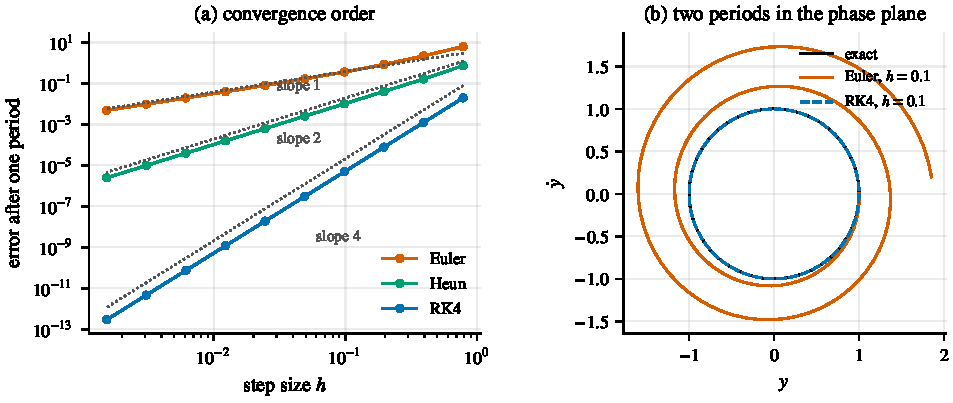
\includegraphics[width=\textwidth]{fig_ode_methods.pdf}
  \caption{Integrating the harmonic oscillator $\ddot y = -y$. (a) Global error after one period versus step size: slopes 1, 2 and 4 confirm the
  orders of Euler, Heun and RK4. (b) With $h = 0.1$, Euler's method spirals outward, gaining energy every step, while RK4 stays on the
  circle to plotting accuracy.}
  \label{fig:ode-methods}
\end{figure}

\paragraph{Verifying the order.} If the error behaves as $Ch^p$, then halving the step divides the error by $2^p$, and the order can be
\emph{measured}: $p \approx \log_2\big(e(h)/e(h/2)\big)$. \Cref{fig:ode-methods}(a) shows this for three methods. A convergence-order test of
this kind is one of the most powerful tests of an integrator: an implementation bug almost always destroys the expected order
(Milestone 4).

\paragraph{Stability.} Euler's method applied to the decaying equation $\dot x = -\lambda x$ gives $x_{k+1} = (1 - h\lambda)x_k$, which blows up
when $h > 2/\lambda$, although the true solution decays. Stiff systems, with very fast decaying modes, need tiny steps or implicit methods.
Applied to an oscillator, Euler's method multiplies the amplitude by $\sqrt{1 + h^2\omega^2} > 1$ per step and spirals outward
(\cref{fig:ode-methods}b). Inertial navigation is not stiff, but this effect is the reason a naive attitude integrator slowly inflates the
norm of its rotation matrix, as we now see.

\subsection{Integrating on a curved space}
\label{sec:lie-euler}

Apply Euler's method to the attitude kinematics $\dot R = R\sx{\omega}$: $R_{k+1} = R_k + hR_k\sx{\omega} = R_k(I + h\sx{\omega})$. The result
is not a rotation matrix:
\begin{equation}
  (I + h\sx{\omega})\T(I + h\sx{\omega}) = I - h^2\sx{\omega}^2 \neq I,
\end{equation}
so every step stretches vectors perpendicular to $\omega$ by a factor of about $1 + \tfrac12h^2\|\omega\|^2$, and the matrix drifts off the set of
rotations. The remedy is to integrate in a way that respects the structure of the space. For constant $\omega$ over the step, the exact
solution is $R_k\exp(h\sx{\omega})$ (\cref{thm:lti-solution}), so the \emph{Lie--Euler} method
\begin{equation}
  R_{k+1} = R_k\exp(h\sx{\omega_k})
\end{equation}
stays exactly on the set of rotations (\cref{prop:exp-skew}) and is first order in general, exact when $\omega$ is constant. Higher-order
generalizations (Runge--Kutta--Munthe-Kaas methods) apply Runge--Kutta to a vector-space parameterization of the increment. Every attitude
update in these notes is multiplicative in this sense (AGENTS.md F1).

% ==============================================================================
\section{Numerical differentiation}
\label{sec:numdiff}

Analytic Jacobians are derived by hand and verified numerically (AGENTS.md E6). Numerical differentiation is easy to write and easy to
get subtly wrong, because it is a subtraction of nearly equal numbers.

\paragraph{Forward differences.} By Taylor's theorem,
\begin{equation}
  \frac{f(x + h) - f(x)}{h} = f'(x) + \frac h2f''(\xi),
\end{equation}
so the \emph{truncation error} is about $\frac h2|f''|$. But $f(x + h)$ and $f(x)$ are each computed with a rounding error of about $u|f|$, and
their difference is divided by $h$, which adds a \emph{rounding error} of about $2u|f|/h$. The total $\frac h2|f''| + \frac{2u|f|}{h}$ is minimized at
$h^\star = 2\sqrt{u|f|/|f''|} \approx 10^{-8}$ for quantities of order one, with a total error of about $10^{-8}$.

\paragraph{Central differences.} Expanding both $f(x \pm h)$,
\begin{equation}
  \frac{f(x + h) - f(x - h)}{2h} = f'(x) + \frac{h^2}{6}f'''(\xi),
\end{equation}
because the even-order terms cancel. The total error $\frac{h^2}6|f'''| + \frac{u|f|}{h}$ is minimized at
\begin{equation}
  h^\star = \left(\frac{3\,u\,|f|}{|f'''|}\right)^{1/3} \approx 10^{-5}\text{ to }10^{-6},
\end{equation}
with a total error of order $u^{2/3} \approx 10^{-11}$.

\begin{figure}[t]
  \centering
  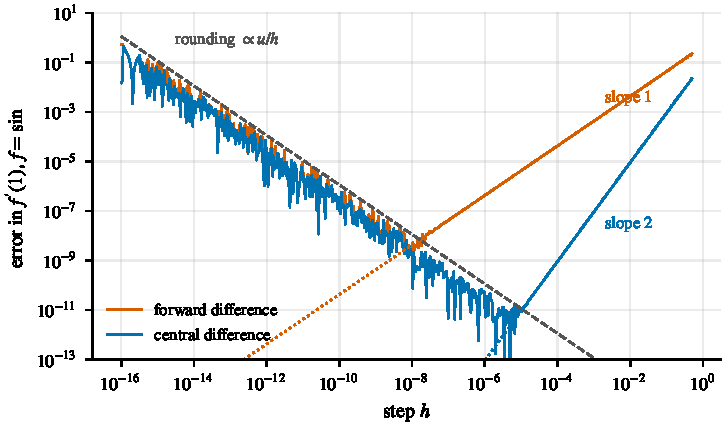
\includegraphics[width=0.85\textwidth]{fig_fd_error.pdf}
  \caption{Error of finite-difference derivatives of $\sin x$ at $x = 1$ versus step size. To the right of the optimum, truncation error
  dominates (slopes 1 and 2); to the left, rounding error grows like $u/h$. Central differences reach about $10^{-11}$; forward differences
  only about $10^{-8}$.}
  \label{fig:fd-error}
\end{figure}

\Cref{fig:fd-error} shows both error regimes. This is why the Jacobian tests of the project use central differences with $h \approx 10^{-6}$
and tolerances of about $10^{-6}$ to $10^{-8}$ relative to the size of the entries. A tolerance tighter than the achievable accuracy makes a
correct implementation fail; a much looser one lets a wrong implementation pass.

\paragraph{Jacobians.} For $f: \R^n \to \R^m$, column $j$ of the numerical Jacobian is
$\big(f(x + he_j) - f(x - he_j)\big)/2h$, costing $2n$ evaluations of $f$. On manifolds the perturbation and the difference are replaced by
$\bplus$ and $\bminus$ (\cref{ch:lie}); nothing else changes.

\begin{aside}[the complex-step derivative]
If $f$ is analytic and can be evaluated with complex arguments, $f'(x) = \operatorname{Im}f(x + ih)/h + O(h^2)$, with no subtraction at all.
With $h = 10^{-20}$ the result is exact to machine precision. The technique requires that every operation in $f$ be implemented for complex
numbers and avoid non-analytic functions (absolute values, comparisons), which rules it out for most estimator code. It is a superb way to
generate reference Jacobians in Python, though.
\end{aside}

\begin{takeaways}
\begin{itemize}
  \item The Jacobian is the matrix of the best linear approximation; the chain rule multiplies Jacobians in composition order.
  \item Taylor's theorem bounds approximation errors. ``First order'' means an error of $O(\|\delta\|^2)$.
  \item $\dd(A\inv) = -A\inv\dd A\,A\inv$ and $\dd\log\det A = \tr(A\inv\dd A)$.
  \item $\dot x = Ax + Bu$ is solved by $e^{At}$ plus a convolution of the inputs; time-varying systems use the state transition matrix,
        which is \emph{not} the exponential of the integrated system matrix unless the matrices commute.
  \item A method of order $p$ has global error $O(h^p)$; halving the step should divide the error by $2^p$. Measure it.
  \item Euler's method leaves the set of rotations; multiplicative updates $R\exp(h\sx{\omega})$ do not.
  \item Central differences with $h \approx 10^{-6}$ reach about $10^{-11}$ accuracy; forward differences only about $10^{-8}$.
\end{itemize}
\end{takeaways}

\begin{exercises}
  \item Compute the Jacobian of $f(x, y) = (x^2y, \sin(xy), e^x)$ and verify it with central differences.
  \item Use Taylor's theorem to bound the error of $\cos h \approx 1 - h^2/2$ for $|h| \le 0.1$.
  \item Show that $\nabla_x\|Ax - b\|^2 = 2A\T(Ax - b)$ and $\nabla_x^2\|Ax - b\|^2 = 2A\T A$.
  \item Solve $\dot x = -2x + 1$, $x(0) = 3$, and check the solution by substitution.
  \item For $A = \begin{bmatrix}0 & 1\\ -1 & 0\end{bmatrix}$, compute $e^{At}$ and interpret the solution of $\dot x = Ax$.
  \item Find the state transition matrix of $\dot x = \begin{bmatrix}0 & t\\0 & 0\end{bmatrix}x$. Do the matrices $A(t)$ commute?
  \item Construct two angular velocity profiles with the same integral $\int\omega\,\dd t$ that produce different final rotations.
  \item Implement Euler, Heun and RK4 for the harmonic oscillator and reproduce \cref{fig:ode-methods}(a).
  \item Show that one Euler step on $\dot R = R\sx{\omega}$ increases $\det R$ by a factor $1 + h^2\|\omega\|^2$, to leading order.
  \item Reproduce \cref{fig:fd-error} and compare the observed optimal step sizes with the formulas of \cref{sec:numdiff}.
\end{exercises}
% Solutions to the exercises of Chapter 4.
\begin{solutions}
  \item Differentiating each component with respect to $x$ and $y$,
        \[
          \frac{\partial f}{\partial(x, y)} = \begin{bmatrix} 2xy & x^2 \\ y\cos(xy) & x\cos(xy) \\ e^x & 0 \end{bmatrix}.
        \]
        At $(x, y) = (0.7, -1.3)$ this is $\begin{bmatrix}-1.82 & 0.49\\ -0.798 & 0.430\\ 2.014 & 0\end{bmatrix}$, and the central-difference Jacobian
        with $h = 10^{-6}$, column $j$ being $\big(f(x + he_j) - f(x - he_j)\big)/2h$, agrees to $10^{-10}$, the accuracy predicted in
        \cref{sec:numdiff}.

  \item The cubic Taylor term of $\cos$ at $0$ vanishes, so $1 - h^2/2$ is also the degree-3 Taylor polynomial, and \cref{thm:taylor} with $n = 3$
        gives the remainder $\cos(\xi)\,h^4/4!$. Hence $|\cos h - (1 - h^2/2)| \le h^4/24 \le 4.2\times10^{-6}$ for $|h| \le 0.1$. The bound is tight:
        at $h = 0.1$ the actual error is $4.165\times10^{-6}$. Using $n = 2$ instead would give the much weaker bound $|h|^3/6 \approx 1.7\times10^{-4}$;
        knowing which terms vanish pays off.

  \item Expand $f(x) = \|Ax - b\|^2 = x\T A\T Ax - 2b\T Ax + b\T b$. The quadratic-form rule with the symmetric matrix $A\T A$ gives
        $\nabla(x\T A\T Ax) = 2A\T Ax$, and $\nabla(b\T Ax) = A\T b$, so
        \[
          \nabla_xf = 2A\T Ax - 2A\T b = 2A\T(Ax - b), \qquad \nabla^2_xf = \frac{\partial}{\partial x}\big(2A\T Ax - 2A\T b\big) = 2A\T A .
        \]
        Setting the gradient to zero gives the normal equations; the Hessian $2A\T A \succeq 0$ shows that any such point is a minimum.

  \item With $a = -2$ and $b = 1$ the integrating-factor formula gives
        \[
          x(t) = 3e^{-2t} + \int_0^te^{-2(t-s)}\,\dd s = 3e^{-2t} + \tfrac12\big(1 - e^{-2t}\big) = \tfrac12 + \tfrac52e^{-2t}.
        \]
        Check: $\dot x = -5e^{-2t}$ and $-2x + 1 = -1 - 5e^{-2t} + 1 = -5e^{-2t}$; $x(0) = \tfrac12 + \tfrac52 = 3$. The solution decays from 3 to the
        equilibrium $\tfrac12$ with time constant $\tfrac12$.

  \item $A^2 = -I$, so as in the solution of Exercise 3.7 the series splits into the cosine and sine series:
        \[
          e^{At} = \cos t\,I + \sin t\,A = \begin{bmatrix}\cos t & \sin t\\ -\sin t & \cos t\end{bmatrix}.
        \]
        This is a rotation by $-t$. The system is $\dot x_1 = x_2$, $\dot x_2 = -x_1$, the harmonic oscillator $\ddot x_1 = -x_1$ with
        $x_1 = \text{position}$ and $x_2 = \text{velocity}$. Its solutions move clockwise around circles at unit angular rate; $\|x\|^2$, the energy, is
        conserved. (Euler's method fails to conserve it, \cref{fig:ode-methods}b.)

  \item The second equation gives $x_2(t) = x_2(s)$, and then $\dot x_1 = t\,x_2(s)$ integrates to $x_1(t) = x_1(s) + \tfrac12(t^2 - s^2)x_2(s)$, so
        \[
          \Phi(t, s) = \begin{bmatrix}1 & \tfrac12(t^2 - s^2)\\ 0 & 1\end{bmatrix}.
        \]
        The matrices do commute: $A(t)A(s) = \begin{bmatrix}0 & t\\0 & 0\end{bmatrix}\begin{bmatrix}0 & s\\0 & 0\end{bmatrix} = 0 = A(s)A(t)$.
        Accordingly property 4 of \cref{prop:stm} applies: $\int_s^tA = \begin{bmatrix}0 & \frac12(t^2 - s^2)\\0 & 0\end{bmatrix}$ is nilpotent and its
        exponential is exactly $\Phi(t, s)$.

  \item Profile A: rotate about $x$ at $\pi/2$~rad/s for one second, then about $y$ at $\pi/2$~rad/s for one second. Profile B: the same two
        segments in the opposite order. Both have $\int\omega\,\dd t = (\pi/2, \pi/2, 0)$. With body rates, $R = R(0)\exp(\cdot)\exp(\cdot)$, so the final
        rotations are
        \[
          R_A = R_x(90^\circ)R_y(90^\circ) = \begin{bmatrix}0 & 0 & 1\\ 1 & 0 & 0\\ 0 & 1 & 0\end{bmatrix}, \qquad
          R_B = R_y(90^\circ)R_x(90^\circ) = \begin{bmatrix}0 & 1 & 0\\ 0 & 0 & -1\\ -1 & 0 & 0\end{bmatrix},
        \]
        both $120^\circ$ rotations but about different axes, $120^\circ$ apart from each other. Neither equals $\exp(\sx{(\pi/2, \pi/2, 0)})$, a
        $127^\circ$ rotation about $(1, 1, 0)/\sqrt2$. The integral of $\omega$ does not determine the rotation; the order of the rotations does.

  \item The implementation follows the formulas of \cref{sec:numint}, with $f(y) = (y_2, -y_1)$, $y_0 = (1, 0)$, and $N$ steps of $h = 2\pi/N$ over one
        period:
\begin{lstlisting}[style=py]
def step(method, y, h):
    f = lambda y: np.array([y[1], -y[0]])
    if method == "Euler": return y + h * f(y)
    if method == "Heun":
        k1 = f(y); k2 = f(y + h * k1); return y + h / 2 * (k1 + k2)
    k1 = f(y); k2 = f(y + h/2 * k1); k3 = f(y + h/2 * k2); k4 = f(y + h * k3)
    return y + h / 6 * (k1 + 2 * k2 + 2 * k3 + k4)
\end{lstlisting}
        The final errors $\|y_N - y_0\|$ for $N = 32, 64, 128, 256$ are $0.84, 0.36, 0.17, 0.080$ (Euler), $4.1\times10^{-2}, 1.0\times10^{-2},
        2.5\times10^{-3}, 6.3\times10^{-4}$ (Heun) and $7.8\times10^{-5}, 4.9\times10^{-6}, 3.0\times10^{-7}, 1.9\times10^{-8}$ (RK4). The ratios between
        successive errors give measured orders $\log_2(e_h/e_{h/2}) \approx 1.1$, $2.0$ and $4.0$. Euler approaches order 1 only slowly because its
        errors are still large: at $N = 32$ the amplitude has already grown by $\big(1 + (2\pi/32)^2\big)^{16} \approx 1.8$.

  \item One Euler step is $R_{k+1} = R_k(I + h\sx{\omega})$, so $\det R_{k+1} = \det R_k\,\det(I + h\sx{\omega})$. The eigenvalues of $\sx{\omega}$ are $0$
        and $\pm i\|\omega\|$ (Exercise 2.7), so those of $I + h\sx{\omega}$ are $1$ and $1 \pm ih\|\omega\|$, and
        \[
          \det(I + h\sx{\omega}) = 1\cdot(1 + ih\|\omega\|)(1 - ih\|\omega\|) = 1 + h^2\|\omega\|^2 .
        \]
        The factor is in fact exact, not only leading order. After $n$ steps $\det R = (1 + h^2\|\omega\|^2)^n \approx e^{nh^2\|\omega\|^2}$: at 200~Hz and
        1~rad/s this is $e^{2.5\times10^{-5}\,n}$, a 2.5\% inflation per thousand steps. The Lie--Euler update $R_k\exp(h\sx{\omega})$ keeps $\det R = 1$ exactly.

  \item Evaluating the two formulas of \cref{sec:numdiff} on a log-spaced grid of $h$ for $f = \sin$ at $x = 1$ reproduces the figure. The theory
        predicts, with $u = 2^{-53}$, $|f| = \sin1 = 0.84$, $|f''| = 0.84$, $|f'''| = \cos1 = 0.54$:
        \begin{itemize}[leftmargin=1.2em]
          \item forward differences: $h^\star = 2\sqrt{u|f|/|f''|} = 2.1\times10^{-8}$, with error $2\sqrt{u|f||f''|} = 1.8\times10^{-8}$;
          \item central differences: $h^\star = (3u|f|/|f'''|)^{1/3} = 8.0\times10^{-6}$, with error $1.7\times10^{-11}$.
        \end{itemize}
        The observed minima (taking the median error in a small window of $h$, since the rounding part is erratic) lie at $h \approx 10^{-8}$ and
        $5\times10^{-6}$, with errors of about $3\times10^{-9}$ and $3\times10^{-12}$. The optimal steps agree with the formulas to within a factor of
        two, and the observed errors are a few times smaller than the predicted ones, because the formulas add worst-case rounding errors while
        the actual rounding errors of $f(x + h)$ and $f(x - h)$ are partly random and partly cancel.
\end{solutions}

